\documentclass[a4paper]{report}
% Shared preamble for the English probability and statistics documents.
% Based on the original course preamble. Compile with pdfLaTeX.
\usepackage[top=1.5cm,bottom=2cm,left=2cm,right=2cm]{geometry}
\usepackage[T1]{fontenc}
\usepackage{lmodern}
\usepackage[utf8]{inputenc}
\usepackage[english]{babel}

\usepackage{amsmath}
\usepackage{amssymb}
\usepackage{amsthm}
\usepackage{mathrsfs}
\usepackage{mathtools}
\usepackage{etoolbox}
\usepackage{tikz}
\usetikzlibrary{shapes.multipart,arrows.meta}
\usepackage{xcolor}
\usepackage{enumerate}
\usepackage[shortlabels]{enumitem}
\usepackage{hyperref}
\usepackage{version}
\usepackage{bbold}
\usepackage{fontawesome5}
\usepackage{fancyhdr}
\lfoot{}
\usepackage{natbib}
\usepackage{graphicx}
\usepackage{pdfpages}
\usepackage{authblk}
    
\usepackage{blindtext}
\usepackage{multicol}
\usepackage{collcell}
\usepackage{wrapfig}
\usepackage{blkarray}
\usepackage{cancel}
\usepackage{appendix}
\usepackage{float}
\makeatletter
\input{tex/assets/slashbox.sty}
\makeatother
\hypersetup{unicode,colorlinks,citecolor=red,filecolor=black,
  linkcolor=red,urlcolor=cyan}
\setlength{\columnsep}{1cm}
\pagenumbering{gobble}

\def\numtext#1{%
  \ifcase#1\or one\or two\or three\or four\or five\or six\or seven\or eight\or nine\or ten\or
  eleven\or twelve\or thirteen\or fourteen\or fifteen\or sixteen\or seventeen\or eighteen\or nineteen\or twenty\or Lots\fi}

\newcommand{\Byte}[1]{%
  \def\nodecontents{}%
  \foreach[count=\l] \k in {#1} {\xappto{\nodecontents}{\noexpand\nodepart{\numtext{\l}}\k}}%
  \node[rectangle split,rectangle split parts=8,rectangle split horizontal,draw] at (2,2){\nodecontents};}

\newcommand{\D}{{\mathrm{d}}}
\newcommand{\cE}{{\mathcal{E}}}
\newcommand{\cG}{{\mathcal{G}}}
\newcommand{\cX}{{\mathcal{X}}}
\newcommand{\cY}{{\mathcal{Y}}}
\newcommand{\cB}{{\mathcal{B}}}
\newcommand{\cF}{{\mathcal{F}}}
\newcommand{\cO}{{\mathcal{O}}}
\newcommand{\cS}{{\mathcal{S}}}
\newcommand{\cT}{{\mathcal{T}}}
\newcommand{\given}{\, \big| \,}
\newcommand{\cL}{{\mathscr{L}}}
\newcommand{\cD}{{\mathcal{D}}}
\newcommand{\cA}{{\mathscr{A}}}
\newcommand{\cP}{{\mathscr{P}}}
\newcommand{\cR}{{\mathscr{R}}}
\newcommand{\A}{{\mathcal A}}
\newcommand{\one}{\mathbb{1}}
\newcommand{\mathbbm}[1]{\mathbb{#1}}

\providecommand{\C}{}
\renewcommand{\C}{\mathbb C}
\newcommand{\R}{\mathbb R}
\newcommand{\Q}{\mathbb Q}
\newcommand{\N}{\mathbb N}
\newcommand{\T}{\mathbb T}
\newcommand{\F}{\mathbb F}
\renewcommand{\P}{\mathbb P}
\newcommand{\Z}{\mathbb Z}
\newcommand{\E}{\mathbb {E}}
\newcommand{\Pbb}[1]{\P\left( #1\right)}
\newcommand{\Ebb}[1]{\E\left[ #1\right]}

\newcommand{\lb}{\left (}
\newcommand{\rb}{\right )}
\newcommand{\lbb}{\left [}
\newcommand{\rbb}{\right ]}
\newcommand{\labs}{\left |}
\newcommand{\rabs}{\right |}
\newcommand{\lbrb}[1]{\lb #1 \rb}
\newcommand{\lbbrbb}[1]{\lbb#1\rbb}
\newcommand{\labsrabs}[1]{\labs#1\rabs}
\newcommand{\lbbrb}[1]{\lbb#1\rb}
\newcommand{\lbrbb}[1]{\lb#1\rbb}
\newcommand{\langlerangle}[1]{\langle#1\rangle}
\newcommand{\lbcurly}{\{}
\newcommand{\rbcurly}{\}}
\newcommand{\curly}[1]{\lbcurly#1\rbcurly}
\newcommand{\abs}{\labsrabs}
\newcommand{\ind}[1]{1_{#1}}
\newcommand{\indep}{\perp \!\!\! \perp}
\renewcommand{\d}{\, \mathrm{d}}

\newtheorem{theorem}{Theorem}
\newtheorem{problemCnt}{Lemma}
\theoremstyle{definition}
\newtheorem{problem}[problemCnt]{Problem}
\newtheorem{problembook}[problemCnt]{\faBook \,  Problem}
\newtheorem{problempencil}[problemCnt]{\faPencil* \,  Problem}
\newtheorem{problemstar}[problemCnt]{\faStar\,  Problem}
\newtheorem{problemstarpencil}[problemCnt]{\faStar \, \faPencil* \,   Problem}
\newtheorem{probleminteresting}[problemCnt]{\faSmile[regular] \,   Problem}
\newtheorem{solution}{Solution}

\newcommand{\fwcell}[1]{\makebox[\arraystretch\normalbaselineskip]{$#1$}}
\newenvironment{enumeratei}{\begin{enumerate}[(i)]}{\end{enumerate}}
\newenvironment{enumeratea}{\begin{enumerate}[(a)]}{\end{enumerate}}
\newenvironment{enumeraten}{\begin{enumerate}[\upshape 1.]}{\end{enumerate}}

% Compatibility helpers needed by a few files in the combined archive.
\AtBeginDocument{\noindent{\footnotesize English translation prepared with ChatGPT (OpenAI, GPT-6), 26 October 2026, for translation of the Bulgarian text into English and LaTeX formatting.
The Bulgarian originals remain the reference; translation may contain errors.}\par\smallskip}
\newcommand{\MissingGraphic}[1]{%
  \begin{center}\fbox{\parbox{0.82\linewidth}{\centering Missing source image: \texttt{#1}}}\end{center}}



\setlength{\emergencystretch}{3em}
\allowdisplaybreaks
\begin{document}


\noindent Software Engineering, 02.02.2026 \hfill Exam

\hrulefill

\begin{it}
The exact grading formula depends on the results. As an approximation, use 2 plus the points earned. Justify every answer with clear, detailed calculations. Electronic devices (except ordinary calculators) and additional materials are prohibited.

Time allowed: 3 hours. Good luck.





\end{it}

\vspace{0.6cm}

\begin{problem} (1 point)
A website randomly displays one of $m$ advertisements whenever the page loads. Let $M$ be the number of advertisements not shown after $n$ loads, and $A$ the event that advertisement 1 has not been shown after $n$ loads. Find $\mathbb P(M=0)$, $\mathbb E[M]$, $\mbox{Var}(M)$, $\mathbb P(M=0|A^c)$ and $\mathbb P(A|M=1)$.
\end{problem}

\vspace{0.2cm}

\begin{problem} (1 point) The number of comments on a popular influencer's latest post is $N\sim\mbox{Po}(120)$. Each comment is positive with probability $30\%$, independently of the others. Let $A$ be the number of positive comments.
\begin{enumerate}
    \item Given exactly $100$ comments, how many do you expect to be positive?
    \item Given exactly $40$ positive comments, what total number of comments do you expect?
    \item What is the correlation between the positive and total comment counts?
    \item Given exactly $120$ comments, approximately what is the probability that the percentage of positive comments differs from 30\% by more than 5 percentage points?
\end{enumerate}
\end{problem}

\vspace{0.2cm}

\begin{problem} (1 point)
In a fictional model, the National Statistical Institute represents quarterly economic growth by a random variable $\Theta$ (in percent). Before collecting data, growth is assumed to fluctuate around zero: $\Theta\sim\mbox{N}(0,4)$. A preliminary report based on incomplete data gives growth $X$. If true growth is $\Theta=\theta$, the preliminary estimate has conditional distribution $X\mid\Theta=\theta\sim\mbox{N}(\theta,1)$.
\begin{enumerate}
    \item Given the preliminary estimate $X=x$, what true growth do you expect and with what uncertainty (variance)?
    \item What is the probability of positive true growth if the preliminary report gives $1\%$?
    \item What is the probability that reported growth is below true growth, given that true growth is positive?
    \item Show that the reporting error $X-\Theta$ and true growth are independent.
\end{enumerate}

\end{problem}

\vspace{0.2cm}

\begin{problem} (1 point)
Let $U_1,U_2$ be independent $\mbox{Unif}(0,1)$ random variables. Put
\[X=U_1-U_2,\qquad Y=|U_1-U_2|, \qquad R=\frac{U_2}{U_1}.\]
Find $f_X$, $\mathbb E[X|U_1>U_2]$, $f_Y$, $\mathbb E[Y]$ and the conditional distribution of $R$ given $U_1>U_2$.
\end{problem}

\pagebreak

\begin{figure}[h]
  \centering
  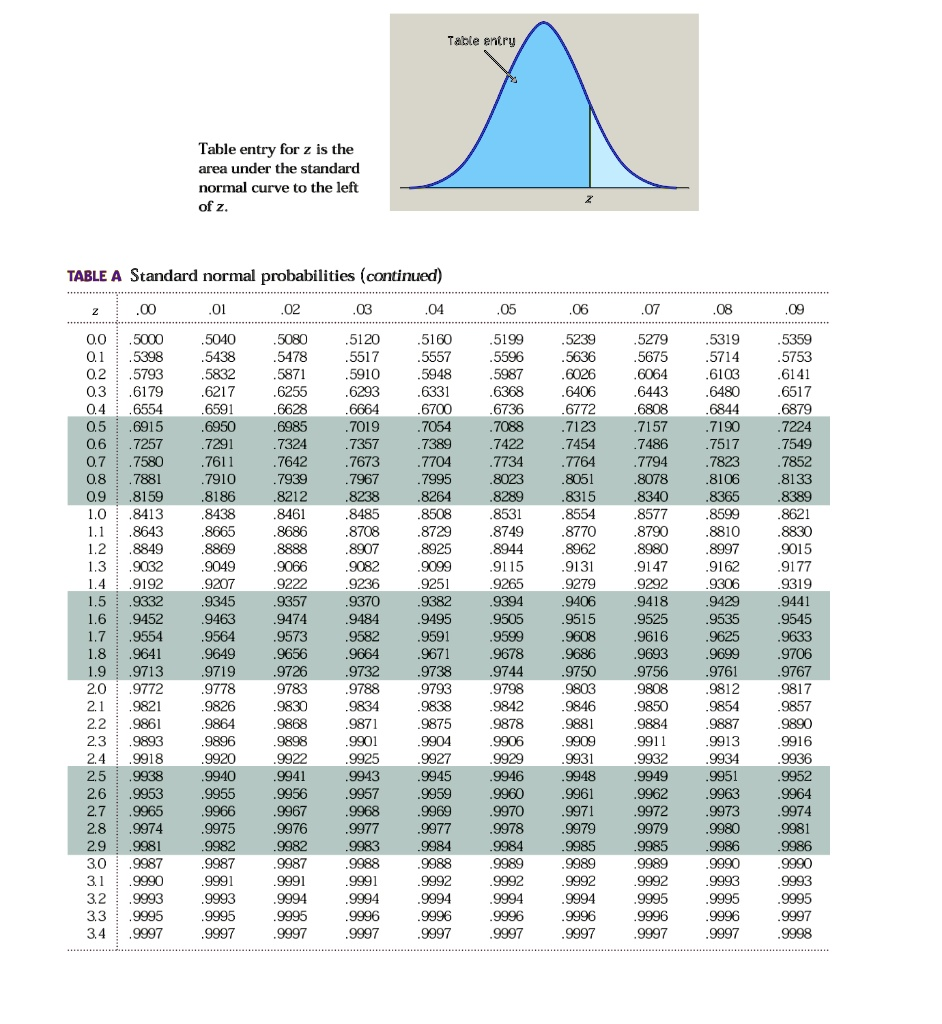
\includegraphics[width=\linewidth]{tex/assets/prob-stat/software-engineering/standard_normal_table.jpg}
\end{figure}

\end{document}
